\documentclass[11pt,a4paper]{article}

\usepackage[english]{babel}
\usepackage[T1]{fontenc}
\usepackage[utf8]{inputenc}
\usepackage{graphicx}
\graphicspath{{../Figs/}}
\usepackage{float}
\usepackage{subcaption}
\usepackage[font=footnotesize,labelfont={sf,bf},textfont=sf,width=\textwidth]{caption}
\usepackage[margin=2cm]{geometry}
\usepackage[plainpages=false,pdfpagelabels,hypertexnames=false]{hyperref}
\usepackage[usenames,dvipsnames]{xcolor}
\usepackage{mathtools}
\usepackage[separate-uncertainty=true]{siunitx}
\usepackage{booktabs}
\usepackage[title]{appendix}

\title{\bfseries\textsc{Hall effect in semiconductors}}
\author{
Michele Masini\\ \small\texttt{\href{mailto:michele.masini@uni-ulm.de}{michele.masini@uni-ulm.de}}\and
Iyán Méndez Veiga\\ \small\texttt{\href{mailto:iyan.mendez-veiga@uni-ulm.de}{iyan.mendez-veiga@uni-ulm.de}}
}
\date{\today}


\begin{document}
\maketitle



\section{Introduction}
In this experiment, we will determine the carrier density ($p$) and the mobility ($\mu$) of a p-type semiconducting sample (Boron) as a function of the temperature, in the range $80K-300K$.

In order to obtain the carrier density we will use Hall-effect. To get the mobility we will measure the resistivity ($\rho$) by means of the van der Pauw method. 

Unfortunately, a semiconducting sample do not have a simple structure and the electric field depends on the position inside the material. This does not allow us to evaluate the Hall coefficient by means of a linear fit between current and voltage. We will show that considering a offset voltage, we will be able to evaluate our coefficient.

In order to evaluate the mobility, we will use the Van der Pauw method. This pysicist proved that we can evaluate the specific resistivity of a sample with an arbitrary shape. Knowing the resistivity and the Hall resistance, we will be able to obtain the mobility. 

\section{Materials and methods}
\subsection{Carrier density}
Let us start explaining the evaluation of the carrier density.

Our sample is under the influence a constant magnetic field ($\vec{B}$). We can evaluate the drift velocity ($\vec{v}_d$) its charge carriers using the equations of motion of a particle in presence of an electric field:
\begin{equation*}
m\frac{d\vec{v}}{dt}+\frac{m}{\tau}\vec{v}_d=-e(\vec{E}+\vec{v}_d\times\vec{B})
\end{equation*} where $\tau$ is called relaxation time. The steady state solution of this equation is: 
\begin{equation}
v_d=-\frac{e\tau}{m}(\vec{E}+\vec{v}_d\times\vec{B})\equiv -\mu (\vec{E}+\vec{v}_d\times\vec{B})
\end{equation}Where $\mu$ is the \emph{mobility}. %In our case the electric field will be parallel to the surface of the sample and the magnetic field orthogonal, hence we can remove the vectors.

Using the definition of density of current in a p-doped matherial: $\vec{j}=ep\vec{v}_d$ (where $e$ is the elementar charge and $p$ is the holes density), we get the following expression for the electric field:
\begin{equation}
\vec{E}=\frac{1}{ep\mu}\vec{j}+\frac{1}{ep}\vec{j}\times\vec{B}\equiv \vec{E}_\parallel+\vec{E}_\perp
\end{equation}

Therefore, measuring the voltage between 2 random points P and N of the sample (as shown in figure {\tiny cite the figure}), what we are obtaining is:
\begin{equation}
U_{PN}=\int_P^N\vec{E}\cdot d\vec{s}=\int_P^{N'}\vec{E}_\perp\cdot d\vec{s}+\int_{N'}^N\vec{E}_\parallel\cdot d\vec{s}
\end{equation}
We will call the second term in the previous expression \emph{offset voltage} ($U_{off}$); this term can be measured in absence of magnetic field. The first term can be evaluated considering that the magnetic field is orthogonal to the sample surface:
\begin{equation}
\int_P^{N'}\vec{E}_\perp\cdot d\vec{s}=-\frac{B}{ep}\int_P^{N'}j\, ds=-\frac{B}{ep}\int_P^{N'}\frac{1}{d}\frac{dI}{ds}\, ds=-\frac{B}{epd}\int_P^{N'} dI=-\frac{BI}{epd}
\end{equation}
Defining $R_H=\frac{1}{ep}$ as the Hall coefficient, we get the relation that will allow us to measure the carrier density:
\begin{equation}
U_{PN}-U_{off}=-R_H\frac{BI}{d}
\end{equation}
\subsection{Mobility}
At this point we will use Van der Pauw method to get the mobility. In 1958 this author (to cite) proved that if we apply a voltage putting sufficently small conctacts at the border of our sample, the sample is homogeneous in thickness ($d$) and it has no isolated holes, then the following formula holds:
\begin{equation}
e^{-\frac{\pi R_{AB,CD}d}{\rho}}+e^{-\frac{\pi R_{BC,DA}d}{\rho}}=1
\end{equation}
where $\rho$ is the resistivity, while $R_{AB,CD}$ is defined as the ratio between the voltage applied between the contact points C and D and the current measured between the points A and B and $R_{BC,DA}$ analogously.

\section{Results and discussion}

\subsection{Calibration of the electromagnet}

We determined the dependence of the magnetic field strength $B$ on the current $I_B$ through the magnetic coils using a calibrated Hall sensor (see Figure \ref{fig:Hall_sensor}).

\begin{figure}[ht]
\centering
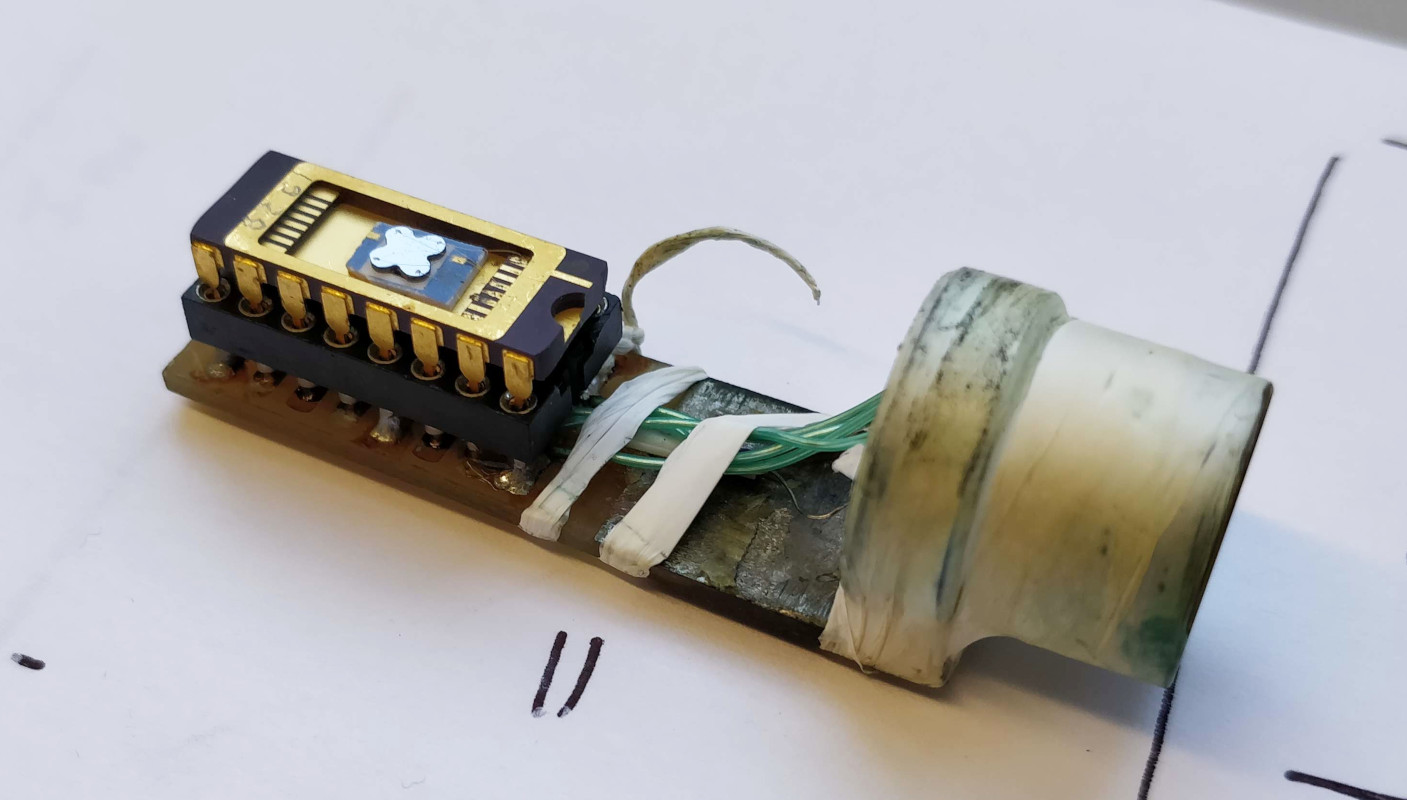
\includegraphics[width=0.6\textwidth]{Hall_sensor}
\caption{Calibrated Hall sensor (\SI{0.1172}{\tesla/\milli\volt} at \SI{10}{\milli\ampere}) used to measure the magnetic field produced by the coils.}
\label{fig:Hall_sensor}
\end{figure}

We measured the voltage for different currents $I_B$ from \SI{0}{\ampere} to \SI{15}{\ampere} in steps of \SI{1}{\ampere} at room temperature ($\sim\SI{300}{\kelvin}$). In Figure \ref{fig:magnetic_field}, the magnetic field computed using the calibration coefficient (see caption Figure \ref{fig:Hall_sensor}) is plotted against the current $I_B$.

\begin{figure}[ht]
\centering
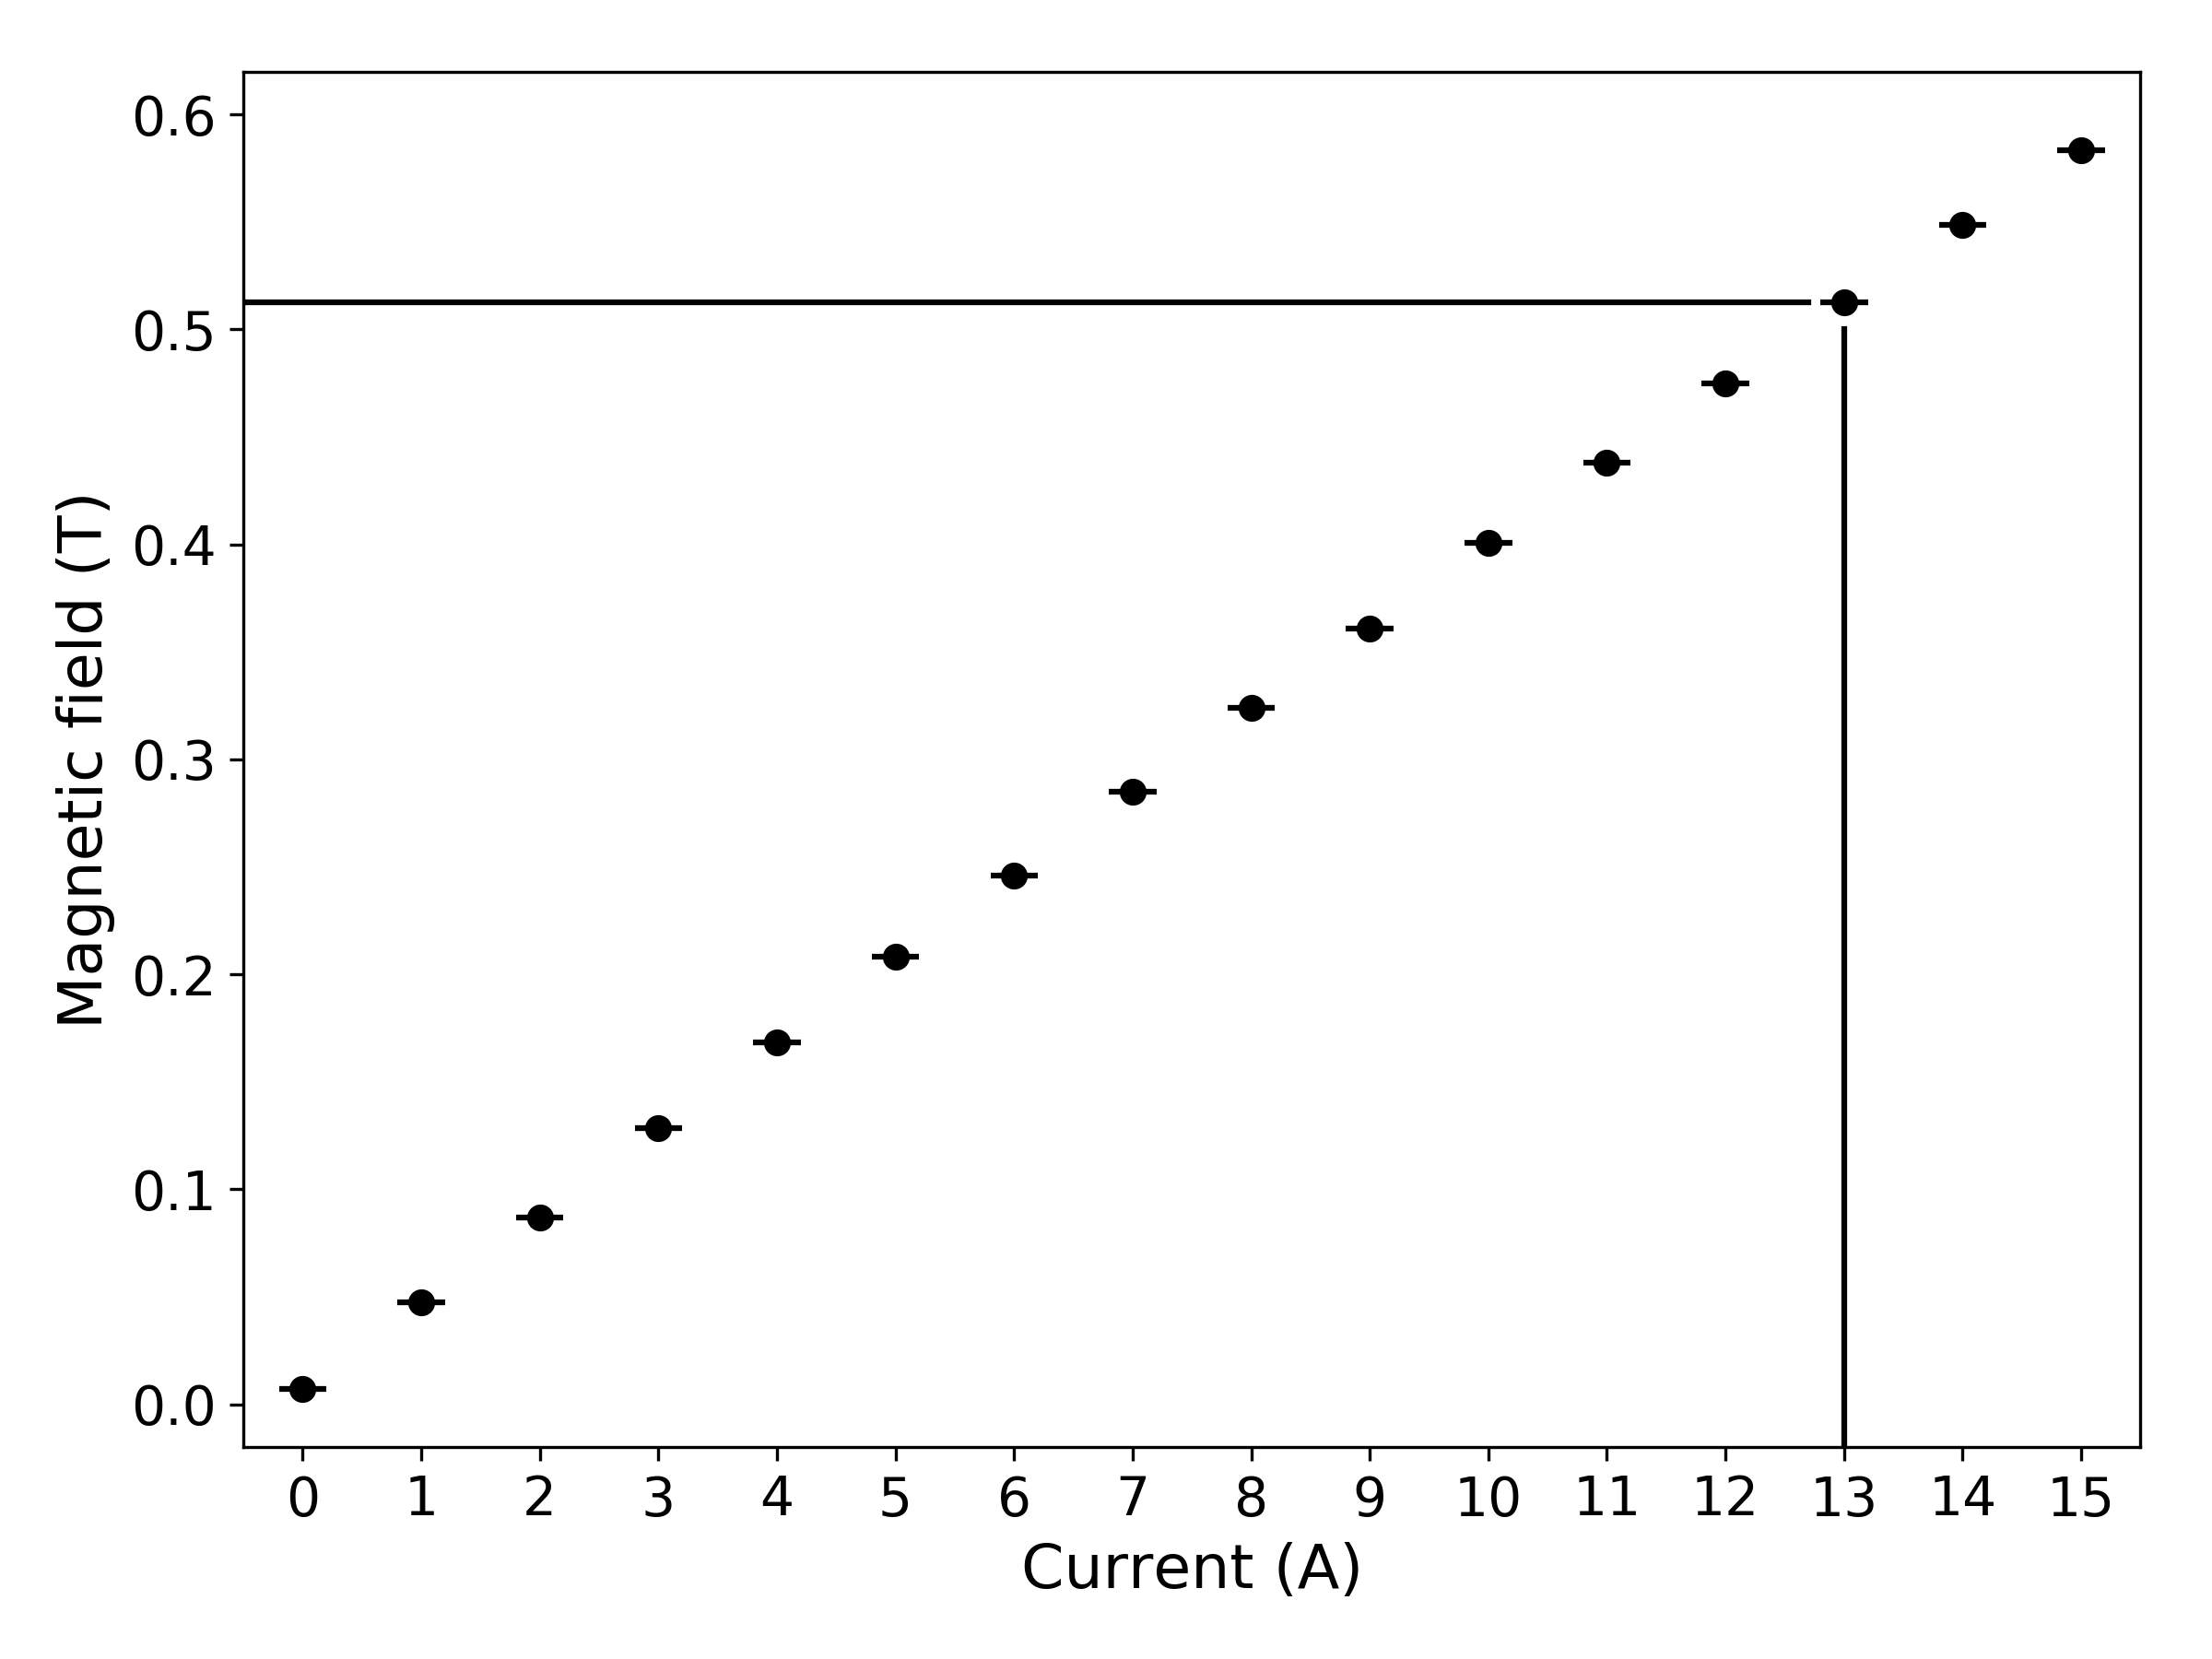
\includegraphics[width=0.8\textwidth]{Magnetic_field_vs_current}
\caption{Magnetic field vs current in the magnetic coils. Solid lines show the current we fixed in the coils for the following measurements, generating a magnetic field of \SI{0.5126}{\tesla}.}
\label{fig:magnetic_field}
\end{figure}

\subsection{Checking ohmic behaviour}

The junction between conductors should have a linear current-voltage curve. We checked this by measuring the voltage between two points for currents from \SI{0}{\micro\ampere} to \SI{150}{\micro\ampere} in steps of \SI{10}{\micro\ampere} also at room temperature. In Figure \ref{fig:ohmic_check}, the linear behaviour is clearly showed.

\begin{figure}[ht]
\centering
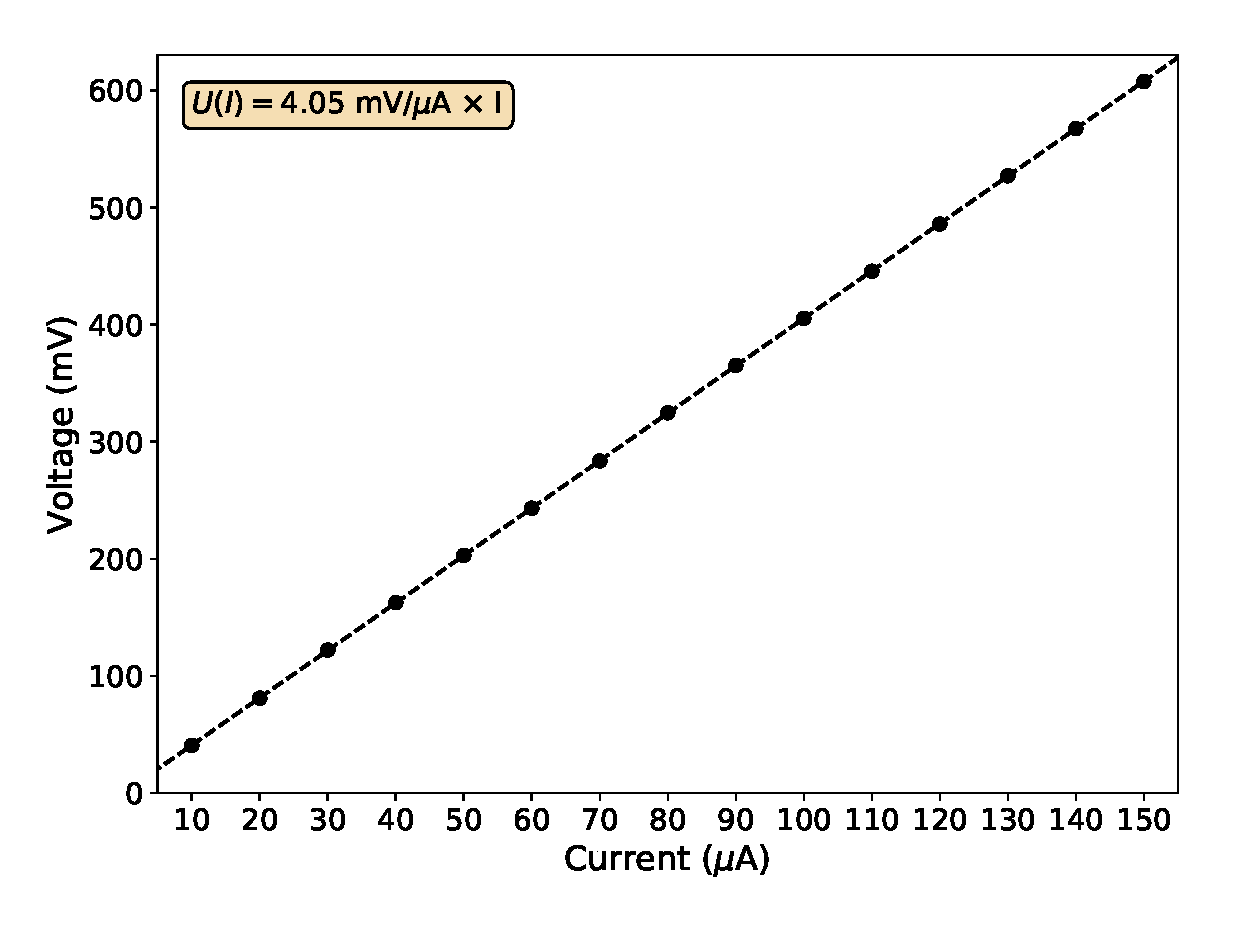
\includegraphics[width=0.8\textwidth]{Voltage_vs_current_ohmic_test}
\caption{Measured voltage vs applied current between two sample contacts. The dashed line is a linear fit of the experimental data with slope \SI{4.05}{\milli\volt/\milli\ampere}.}
\label{fig:ohmic_check}
\end{figure}

\subsection{Orientation of the sample}

In order to align the sample perpendicular to the magnetic field generated by the coils, we measured the transverse voltage $U_t$, i.e. the Hall voltage plus the offset voltage (see {\color{red}Reference theory or figure}), with a fixed magnetic field $B=\SI{0.5126}{\tesla}$ and current $I=\SI{100}{\micro\ampere}$ for different angles between the magnetic field and the surface normal of the sample from \ang{-90} to \ang{90} in steps of \ang{10}.

\begin{figure}[ht]
\centering
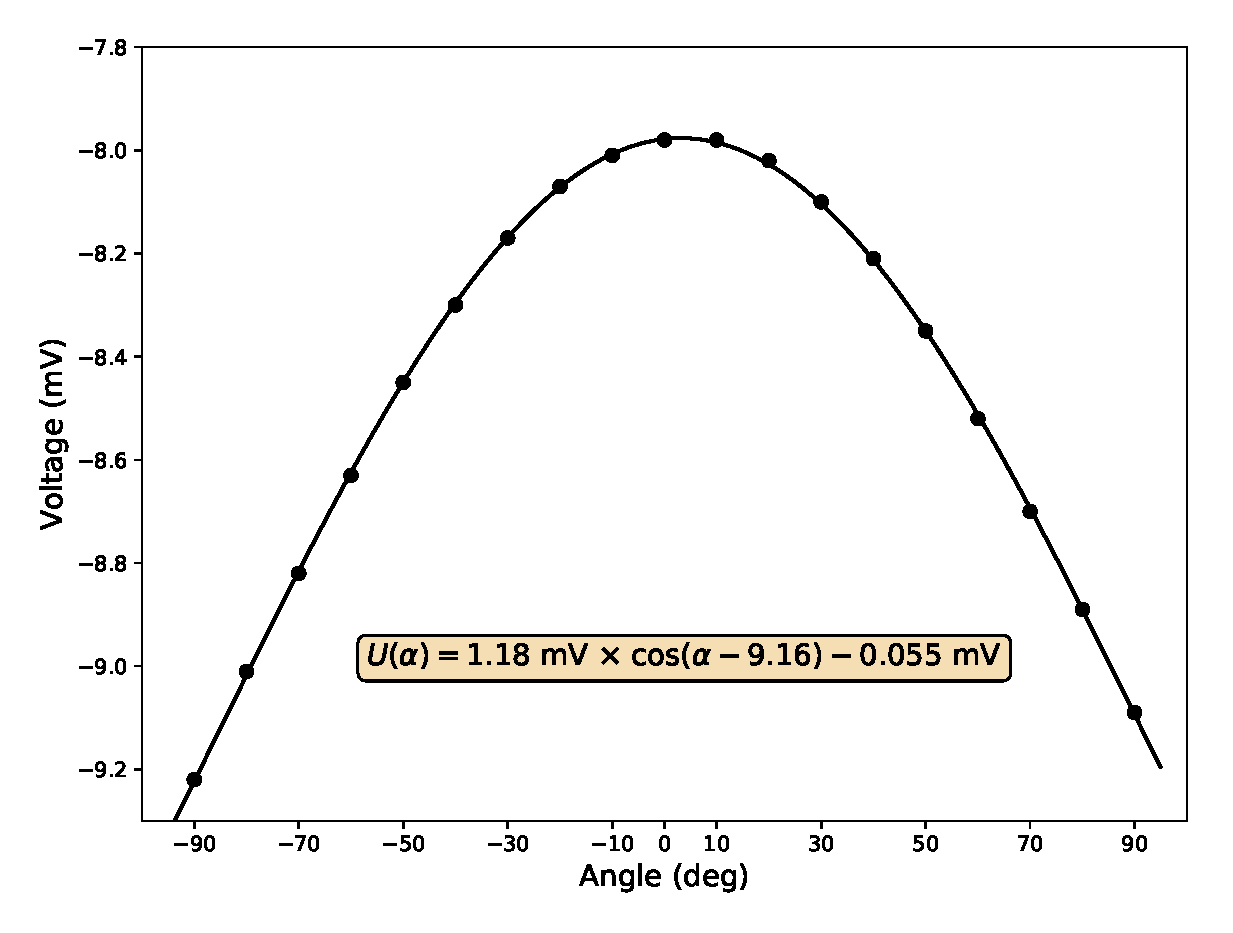
\includegraphics[width=0.8\textwidth]{Voltage_vs_angle}
\caption{Transverse voltage vs orientation angle of the sample with respect to the applied magnetic field. Dash line is a fit using the function $U_t(\alpha)=U_0\cos(\alpha+\phi) + U_\text{off}$. Values obtained for the fitting parameters are shown in the plot box.}
\label{fig:orientation}
\end{figure}

\section{Conclusions}

%\nocite{*}
%\vfill
%\bibliographystyle{unsrt}
%\bibliography{references}

\begin{appendices}


\end{appendices}
\end{document}